\section{Monoidal objects in iconic tricategories}
\label{sec:mono-objects}

[TODO: Work this together.  Perhaps use locally cubical bicategories instead.]

We can define symmetric, braided and monoidal structure of objects, 1-cells and 2-cells internal to an iconic tricategory with products. 
We do this by taking the definitions of monoidal, braided, and symmetric structure given in ~\cite{nick:tricatsbook}, ~\cite{mccrudden:bal-coalgb}, and ~\cite{gg:ldstr-tricat}, but regard the required data abstractly as data about objects, 1-cells, 2-cells, and 3-cells in an iconic tricategory. 

\begin{defn}
A {\bf monoidal object} in an iconic tricategory with products is an object $A$, equipped with 1-cells $\otimes_A: A \times A \rightarrow A$ and $I_A: * \rightarrow A$, and 2-cells
\begin{itemize} 
\item $\alpha: \otimes \odot (\id \times \otimes) \Rightarrow \otimes \odot (\otimes \times \id)$
\item $l: \otimes \odot (I \times \id) \Rightarrow \id$ and $r:\otimes \odot (\id \times I) \Rightarrow \id$ 
\end{itemize}
Finally, it must be equipped with the invertible 3-cells $\pi, \mu, \lambda, \rho$, relating the two different ways around the Mac Lane pentagon and the three other coherence diagrams given in Definition 4.1 of ~\cite{nick:tricatsbook}, which satisfy the three commutativity axioms. 

A monoidal object is {\bf braided} if in addition there is a 2-cell $\sigma_A: \otimes \Rightarrow \otimes \circ \tau$, where $\tau: A \times A \rightarrow A \times A$ interchanges the two copies of $A$; and if there are invertible 3-cells 

\begin{equation}
  \begin{aligned}
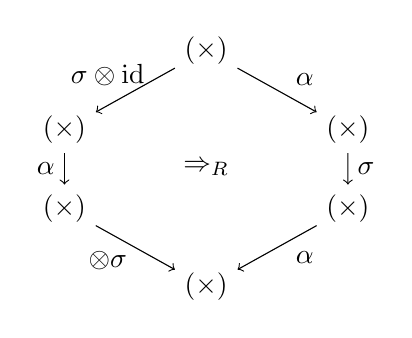
\begin{tikzpicture}[xscale=0.9]
\node (t) at (2,3) {$\ten (\ten \times \id)$};
\node (tl) at (0,2) {$\ten(\ten \times \id)$};
\node (bl) at (0,1) {$\ten (\id \times \ten)$};
\node (b) at (2,0) {$\ten (\id \times \ten)$};
\node (tr) at (4,2) {$\ten(\id \times \ten)$};
\node (br) at (4,1) {$\ten (\ten \times \id)$};
\draw[->] (t) to node [above,xshift=10pt, yshift=-2] {$\alpha$} (tr);
\draw[->] (tr) to node [right] {$\sigma$} (br);
\draw[->] (br) to node [below,xshift=10pt, yshift=2pt] {$\alpha$} (b);
\draw[->] (t) to node [above,xshift=-10pt, yshift=-2pt] {$\sigma \otimes \mbox{id}$} (tl);
\draw[->] (tl) to node [left] {$\alpha$} (bl);
\draw[->] (bl) to node [below,xshift=-10pt,yshift=2pt] {$\mathid \otimes \sigma$} (b);
\node at (2,1.5) {$\Rightarrow_{R \iso}$};
\end{tikzpicture}
  \end{aligned}
\hspace{5pt}\mbox{and} \hspace{5pt}
\begin{aligned}
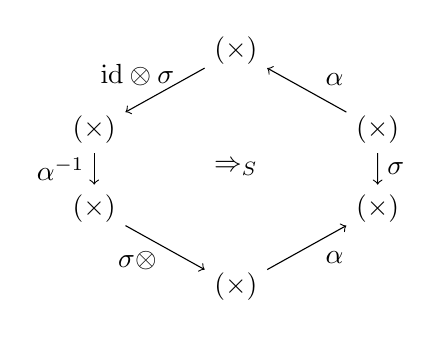
\begin{tikzpicture}[xscale=0.9]
\node (t) at (2,3) {$\ten(\id \times \ten)$};
\node (tl) at (0,2) {$\ten(\id \times \ten)$};
\node (bl) at (0,1) {$\ten(\ten \times \id)$};
\node (b) at (2,0) {$\ten(\ten \times \id)$};
\node (tr) at (4,2) {$\ten(\ten \times \id)$};
\node (br) at (4,1) {$\ten(\id \times \ten)$};
\draw[->] (tr) to node [above,xshift=10pt, yshift=-2] {$\alpha$} (t);
\draw[->] (tr) to node [right] {$\sigma$} (br);
\draw[->] (b) to node [below,xshift=10pt, yshift=2pt] {$\alpha$} (br);
\draw[->] (t) to node [above,xshift=-10pt, yshift=-2pt] {$\mbox{id} \otimes \sigma$} (tl);
\draw[->] (tl) to node [left] {${\alpha}^{-1}$} (bl);
\draw[->] (bl) to node [below,xshift=-10pt,yshift=2pt] {$\sigma \otimes \mathid$} (b);
\node at (2,1.5) {$\Rightarrow_{S \iso}$};
\end{tikzpicture}
\end{aligned}
\end{equation}
satisfying the axioms (BA1), (BA2), (BA3), and (BA4) given in ~\cite[p136--139]{mccrudden:bal-coalgb} . 
It is {\bf sylleptic} when there exists an invertible 3-cell

 \[
 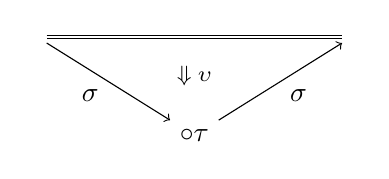
\begin{tikzpicture}
 \node (tl) at (-2,1) {$\ten$};
 \node (tr) at (2,1) {$\ten$};
 \node (b) at (0,-.25) {$\ten \circ \tau$};
 \draw[double] (tl)  -- (tr);
 \draw[->] (tl) to node[left, yshift=-5pt]{$\sigma$} (b);
 \draw[->] (b) to node[right, yshift=-5pt] {$\sigma$}(tr);
 \node at (0,0.5) {\footnotesize $\Downarrow \upsilon \iso$}; 
 \end{tikzpicture}
 \]
  satisfying the axioms (SA1), (SA2) on~\cite[p144--145]{mccrudden:bal-coalgb}. It is {\bf symmetric} if in addition, it satisfies the axiom given on~\cite[p91]{mccrudden:bal-coalgb}.
\end{defn}


\begin{defn}
Let $A,B$ be monoidal objects in an iconic tricategory  with products. A 1-cell $f:A \rightarrow B$ is {\bf lax monoidal} when it is equipped with the following 2-cells:
\begin{itemize}
\item $\chi: \otimes_B \odot (f,f) \Rightarrow f \odot \otimes_A$
\item $\iota: I_B \Rightarrow f \odot I_A$
\end{itemize}
As well as invertible 3-cells $\omega, \gamma$, and $\delta$ given in Definition 4.10 of ~\cite{nick:tricatsbook}, expressing the usual associativity and unitality conditions, which satisfy the two given commutativity axioms.
A monoidal 1-cell is called {\bf braided}, when $A$ and $B$ are braided and there is a 2-cell $u: \sigma_B \odot \chi  \Rightarrow \chi \odot f\sigma_A$, satisfying the braiding axioms analogous to (BHA1) and (BHA2) given in  \cite[p141-142]{mccrudden:bal-coalgb}. It is {\bf symmetric} when $A$ and $B$ are symmetric and the 3-cells defining the braided monoidal structure of $f$ satisfy the additional axiom analogous to  (SHA1) given in   \cite[p145]{mccrudden:bal-coalgb}.

When the natural transformations are in the opposite direction, the functor is {\bf oplax monoidal}, and when they are isomorphisms, the functor is {\bf strong monoidal}.
\end{defn}



\begin{defn}\label{Def:monverttrans}
Let $f, g:A \rightarrow B$ be monoidal 1-cells in a tricategory with products. A {\bf monoidal 2-cell} $\alpha: f \Rightarrow g$ is equiped with 3-cells
\begin{itemize}
\item $\Pi: \chi_f \odot \alpha \Rightarrow (\alpha \otimes \alpha) \odot \chi_g$
\item $M: \iota_f \odot \alpha \Rightarrow \iota_g$
\end{itemize}
such that the three coherence axioms in definition 3 of ~\cite{gg:ldstr-tricat} hold.
A monoidal 2-cell is {\bf braided} or {\bf symmetric} when $f,g$ are braided or symmetric, and in addition the additional coherence axiom analogous to (BTA1) of ~\cite[p143]{mccrudden:bal-coalgb} holds. Note that here the author writes $\rho$ for our braiding 1-cell $\sigma$.
\end{defn}


